\chapter{Système d'exploitation}

%TODO explication OS autoscope, yocto, linux raspi

\section{Support de la caméra}

Pour gérer les différentes configurations matérielles de façon plus "userfriendly", la Raspberry-Pi dispose d'un fichier de configuration \codeinline{text}{config.txt} que le $bootloader$ interprétera pour sélectionner les $overlays$ correspondants et composer le $devicetree$ qui convient à l'architecture matérielle utilisée. Celui-ci étant ensuite passé au $kernel$ lors du démarrage.

%\vspace{1cm}

Cette subtilité propre aux Raspberry-Pi permet à l'utilisateur de ne pas avoir besoin d'avoir affaire au $devicetree$ quand il s'agit de configuration. Par exemple l'activation du support d'un élément courant sur les Raspberry-Pi comme le module Raspicam.

%\vspace{1cm}

le logiciel \codeinline{text}{raspi-config} n'est autre qu'une interface à ce fichier de configuration.

\vspace{1cm}

Pour activer le support matériel de la caméra, il faut ajouter les lignes suivantes à ce fichier~:

%\code{ruby}
\code{bash}
start_x=1
gpu_mem=128
\end{minted}

%À travers Yocto, cela passe par l'ajout des lignes ci-dessous au fichier \codeinline{text}{local.conf} et donc à son modèle le fichier \codeinline{text}{meta-autoscope/conf/local.conf.sample} dans la $layer$ dédiée au projet.

À travers Yocto, le fichier \codeinline{text}{config.txt} est généré par la recette\\\codeinline{text}{meta-raspberrypi/recipes-bsp/bootfiles/rpi-config_git.bb}.

On la surcharde donc, dans la $layer$ dédiée au projet, de la recette\\\mintinline[fontsize=\footnotesize]{text}{meta-autoscope/recipes-bsp/bootfiles/rpi-config_%.bb}~:

\code{bash}
VIDEO_CAMERA = "1"
GPU_MEM = "128"
\end{minted}

\vspace{1cm}

Quant à l'utilisation de la caméra, il existe des logiciels tels que \codeinline{text}{raspivid} pour filmer ou \codeinline{text}{raspistill} pour prendre des clichés. Tous deux font partie de la suite \codeinline{text}{userland} que l'on ajoute à notre image via la ligne ci-dessous dans le fichier\\\codeinline{text}{meta-autoscope/recipes-autoscope/images/autoscope-console-image.bb}~:

\code{bash}
IMAGE_INSTALL += "userland"
\end{minted}

À l'usage, la commande suivante permet d'afficher en plein écran le flux vidéo jusqu'à ce qu'on le stoppe~:

\code{text}
root@autoscope ~ #
    raspivid -t 0
\end{minted}

\section{Étude du transfert du flux vidéo sur le réseau} %TODO python hélice

Pour l'instant seul un test a été réalisé. Il s'agit d'afficher sur un ordinateur distant le flux vidéo filmé par la Raspberry-Pi. On utilise pour cela \codeinline{text}{netcat}.

\code{text}
~ $
    nc -l -p 5001 | /usr/bin/mplayer -fps 10 -cache 1024 -

root@autoscope ~ #
    raspivid -fps 10 -t 0 -o - | nc <ip.de.l'ordinateur> 5001
\end{minted}

\vspace{1cm}

La procédure fonctionne, le lecteur \codeinline{text}{mplayer} s'ouvre et lit la vidéo, toutefois malgré le taux de rafraîchissement très faible ($10fps$), une latence particulièrement longue existe, de l'ordre de 2 à 10 secondes.

D'autres solutions plus performantes existent sûrement, en particulier des solutions de plus bas niveau intégrables à un programme C ou C++.

\section{Splash screen}

Le système d'exploitation disposait déjà d'un écran de démarrage aux couleurs de l'école survenant lors de la phase d'initialisation du système.

Un second a été ajouté lors de la phase précédente, le démarrage du kernel, c'est à dire de Linux. Cela n'a pas vraiment d'intérêt pour le télescope si ce n'est un peu d'esthétique lorsqu'il démarre avec un écran branché. Cependant cela met en œuvre un processus qui sera utile pour d'autres choses, la configuration du kernel.

\vspace{1cm}

Les éléments des sources de Linux impliqués dans le splash screen sont les suivants~:
\begin{itemize}[label=$\bullet$]
	\item Dans le dossier \codeinline{text}{kernel-source/drivers/video/logo/}
	\begin{itemize}
		\item \codeinline{text}{Makefile}
		\item \codeinline{text}{Kconfig}
		\item \codeinline{text}{logo.c}
		\item Différents fichiers image, ceux nous intéressant sont au format \codeinline{text}{logo_*_clut224.ppm}
		\end{itemize}
	\item Dans le dossier \codeinline{text}{kernel-source/include/linux/}
	\begin{itemize}
		\item \codeinline{text}{linux_logo.h}
		\end{itemize}
	\end{itemize}

\vspace{1cm}

Tout d'abord l'on crée une recette yocto de surcharge de la recette kernel utilisée par la \codeinline{text}{meta-raspberrypi}. Voici l'allure du dossier associé à la recette. À noter que l'arborescence utilisée par une recette de surcharge du kernel est plus sensible qu'une recette de surcharge quelconque.

\code{text}
~/yocto/sources/meta-autoscope $ tree recipes-kernel/
    recipes-kernel/
    └── linux/
        ├── linux-raspberrypi/
        │   └── raspberrypi3/
        └── linux-raspberrypi_%.bbappend
\end{minted}

\vspace{1cm}

Ensuite l'on crée l'image qui servira d'écran de démarrage, en commencant par lui donner les dimensions souhaitées, ici $1822\times 900$. Il faut alors la convertir au format qui convient~:

\code{text}
jpegtopnm lune-1822x900.jpg | ppmquant 224 | pnmnoraw > logo_autoscope_clut224.ppm 
mv logo_autoscope_clut224.ppm ~/yocto/sources/meta-autoscope/recipes-kernel/linux/linux-raspberrypi/raspberrypi3/
\end{minted}

\vspace{1cm}

Puis des lignes sont à ajouter dans les sources du kernel dont la localisation dans l'arborescence yocto est la suivante~:
\codeinline{text}{~/yocto/build/tmp/work-shared/raspberrypi3/kernel-source/}

\vspace{1cm}

\codeinline{text}{include/linux/linux_logo.h}~:
\code{C}
extern const struct linux_logo logo_autoscope_clut224;
\end{minted}

%\vspace{1cm}

\codeinline{text}{drivers/video/logo/logo.c}~:
\code{C}
#ifdef CONFIG_LOGO_AUTOSCOPE_CLUT224
        /* Autoscope Linux logo */
        logo = &logo_autoscope_clut224;
#endif
\end{minted}

%\vspace{1cm}

\codeinline{text}{drivers/video/logo/Makefile}~:
\code{makefile}
obj-$(CONFIG_LOGO_AUTOSCOPE_CLUT224)    += logo_autoscope_clut224.o
\end{minted}

%\vspace{1cm}

\codeinline{text}{drivers/video/logo/Kconfig}~:
\code{kconfig}
config LOGO_AUTOSCOPE_CLUT224
    bool "224-color Autoscope Linux logo"
    default y

\end{minted}

%\vspace{1cm}

On réalise un patch de ces modifications~:

\code{text}
~/yocto/build/tmp/work-shared/raspberrypi3/kernel-source $
    git add drivers/video/logo/{Kconfig,Makefile,logo.c} incude/linux/linux_logo.h
    git commit -m "Autoscope logo"
    git format-patch -1
    mv 0001-Autoscope-logo.patch ~/yocto/sources/meta-autoscope/recipes-kernel/linux/linux-raspberrypi/raspberrypi3/
\end{minted}

\vspace{1cm}

On configure ensuite le kernel afin d'activer l'écran de démarrage et de choisir celui souhaité. On réalise pour cela un $fragment$ de configuration~:

\codeinline{text}{meta-autoscope/recipes-kernel/linux/linux-raspberrypi/raspberrypi3/logo.cfg}~:
\code{C}
CONFIG_LOGO=y
CONFIG_LOGO_LINUX_MONO=y
CONFIG_LOGO_LINUX_VGA16=y
# CONFIG_LOGO_LINUX_CLUT224 is not set
CONFIG_LOGO_AUTOSCOPE_CLUT224=y
\end{minted}

\vspace{1cm}

La dernière étape est d'écrire la recette pour prendre en compte toutes ces modifications~:

\codeinline{text}{meta-autoscope/recipes-kernel/linux/linux-raspberrypi_\%.bbappend}~:
\code{bash}
FILESEXTRAPATHS_prepend := "${THISDIR}/${PN}:"

SRC_URI_append_raspberrypi3 += " \
    file://0001-Autoscope-logo.patch \
    file://logo.cfg \
    file://logo_autoscope_clut224.ppm \
    "

do_patch_prepend() {
    cp ${WORKDIR}/logo_autoscope_clut224.ppm ${S}/drivers/video/logo/
}
\end{minted}

\vspace{1cm}
Voici donc l'arborescence associée à la recette~:

\code{text}
~/yocto/sources/meta-autoscope $ tree recipes-kernel/
    recipes-kernel/
    └── linux/
        ├── linux-raspberrypi/
        │   └── raspberrypi3/
        │       ├── 0001-Autoscope-logo.patch
        │       ├── logo_autoscope_clut224.ppm
        │       └── logo.cfg
        └── linux-raspberrypi_%.bbappend
\end{minted}

\vspace{1cm}

Après une longue phase de compilation puisque le kernel est recompilé, on observe au démarrage la succession des deux écrans de démarrages~:

\begin{figure}[H]
    \centering
    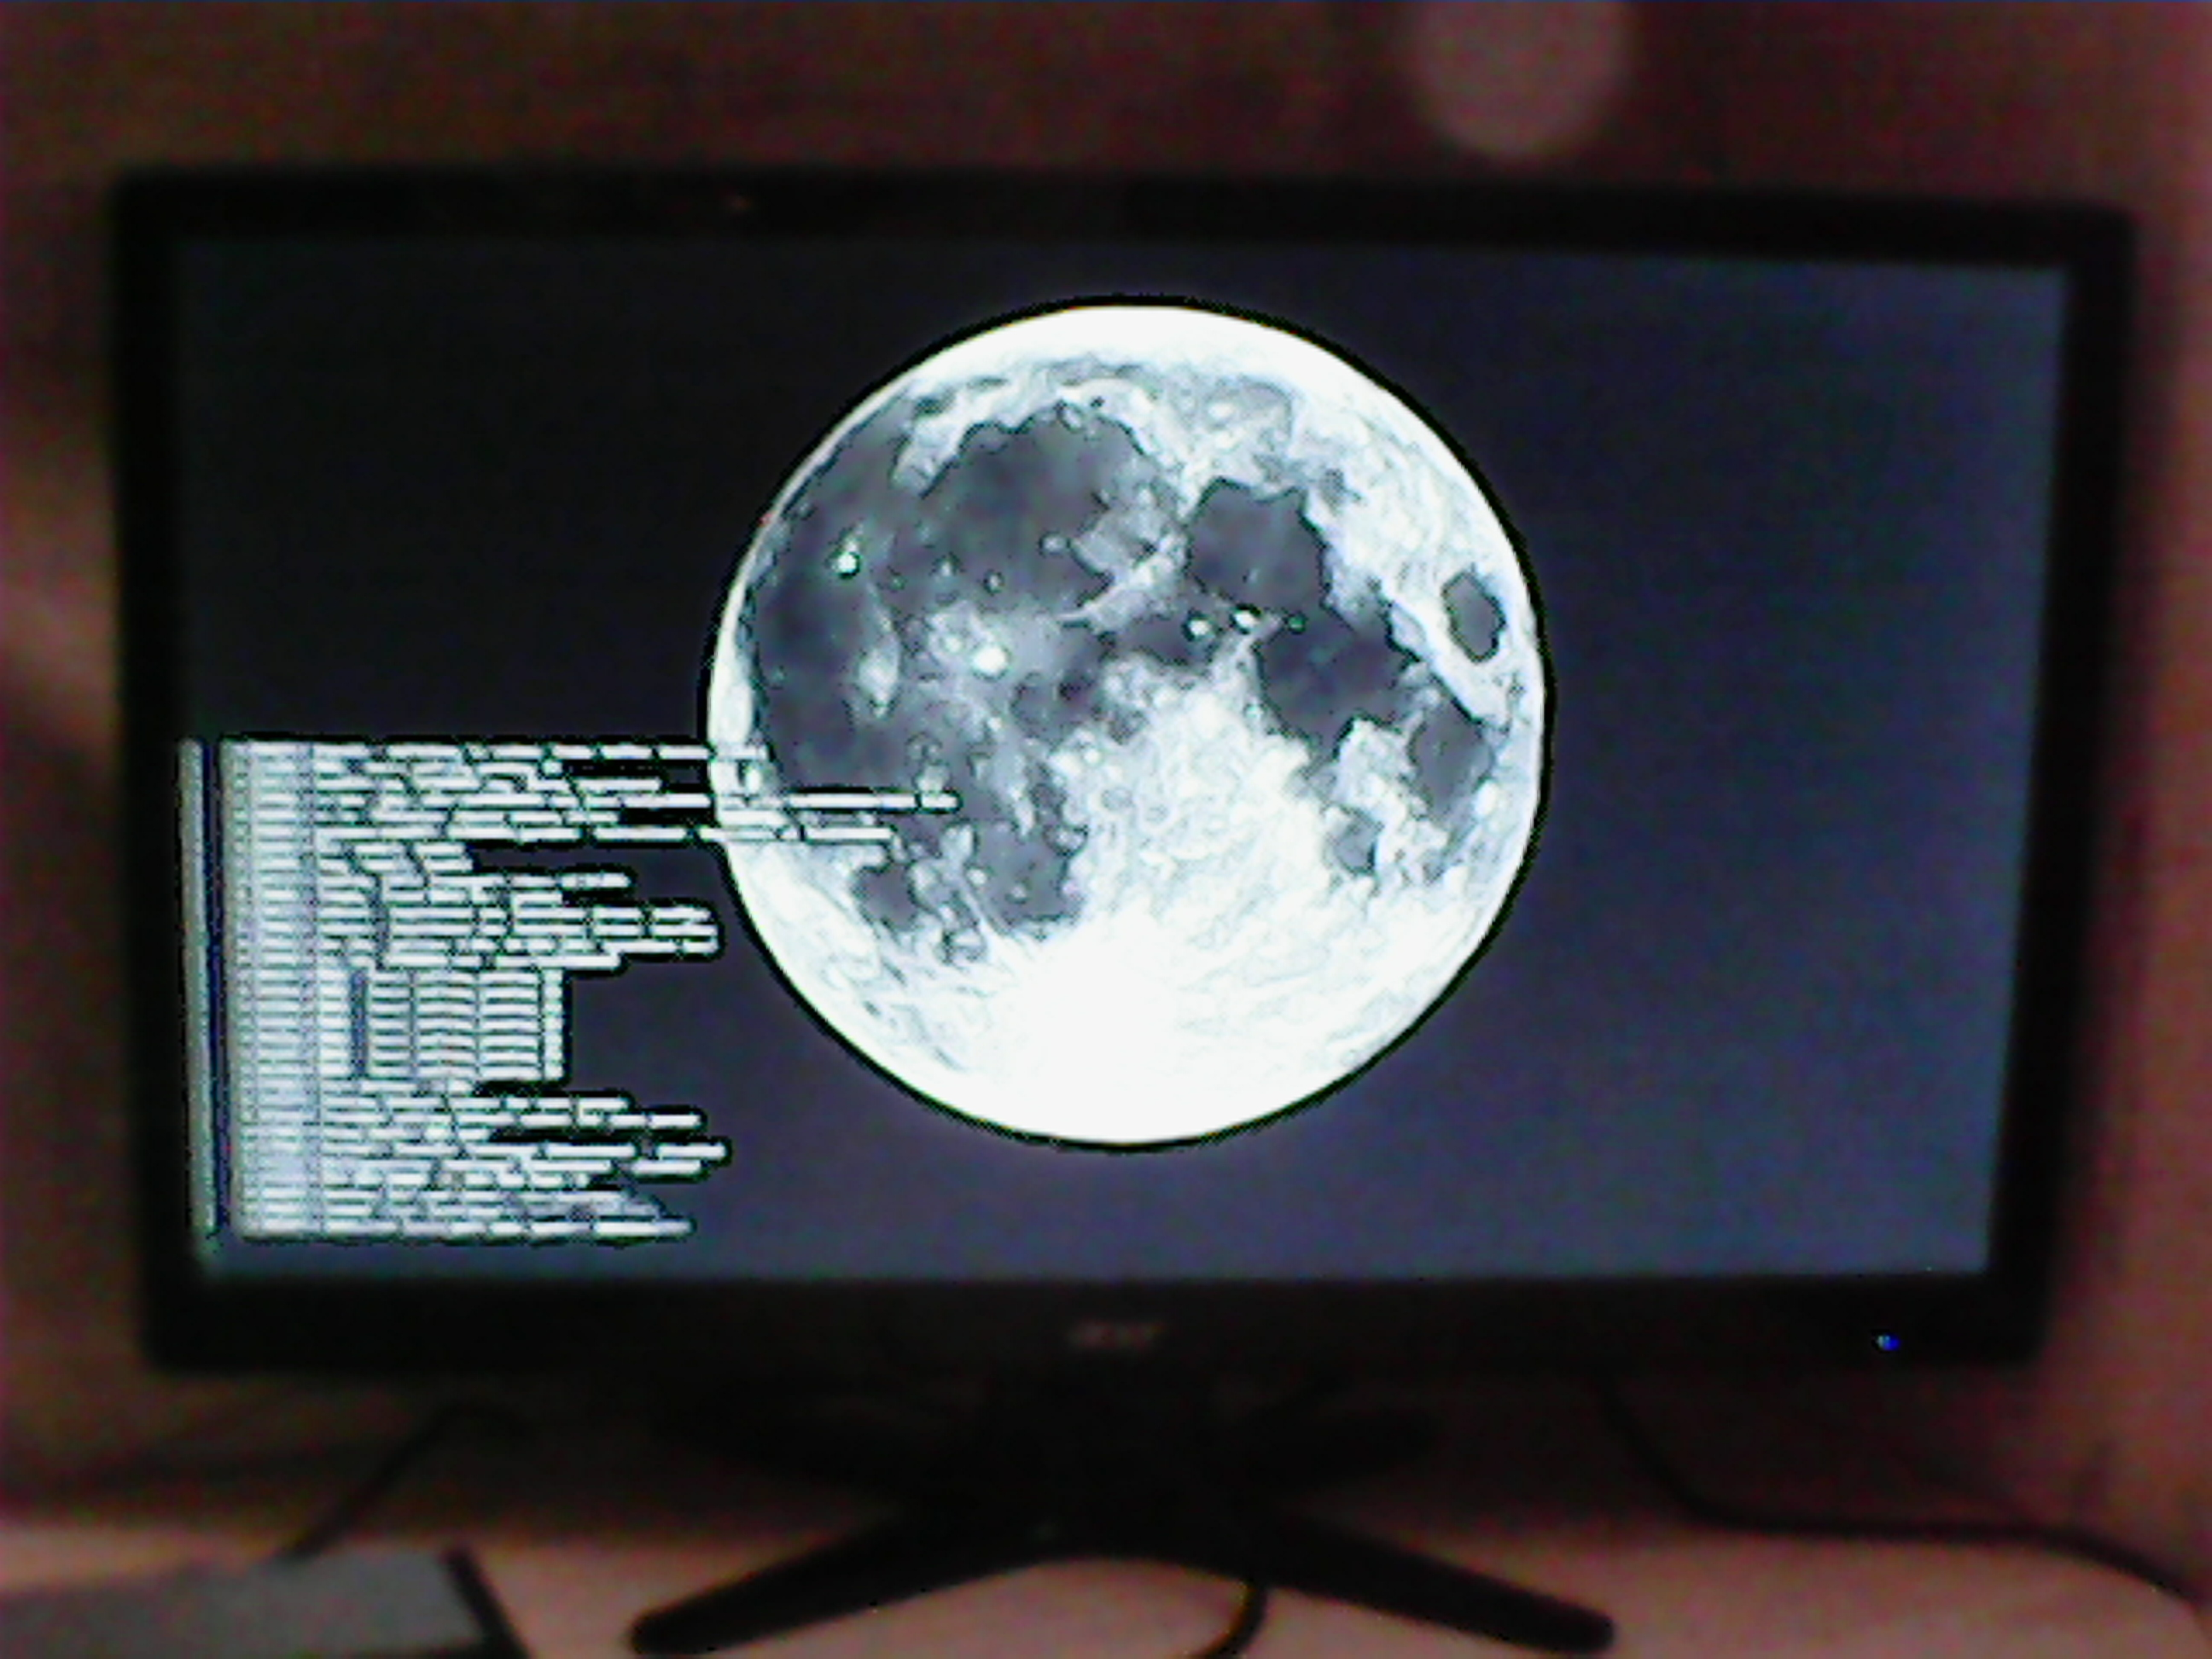
\includegraphics[width=0.49\linewidth]{\figures/photo_splashk_2.jpg}
    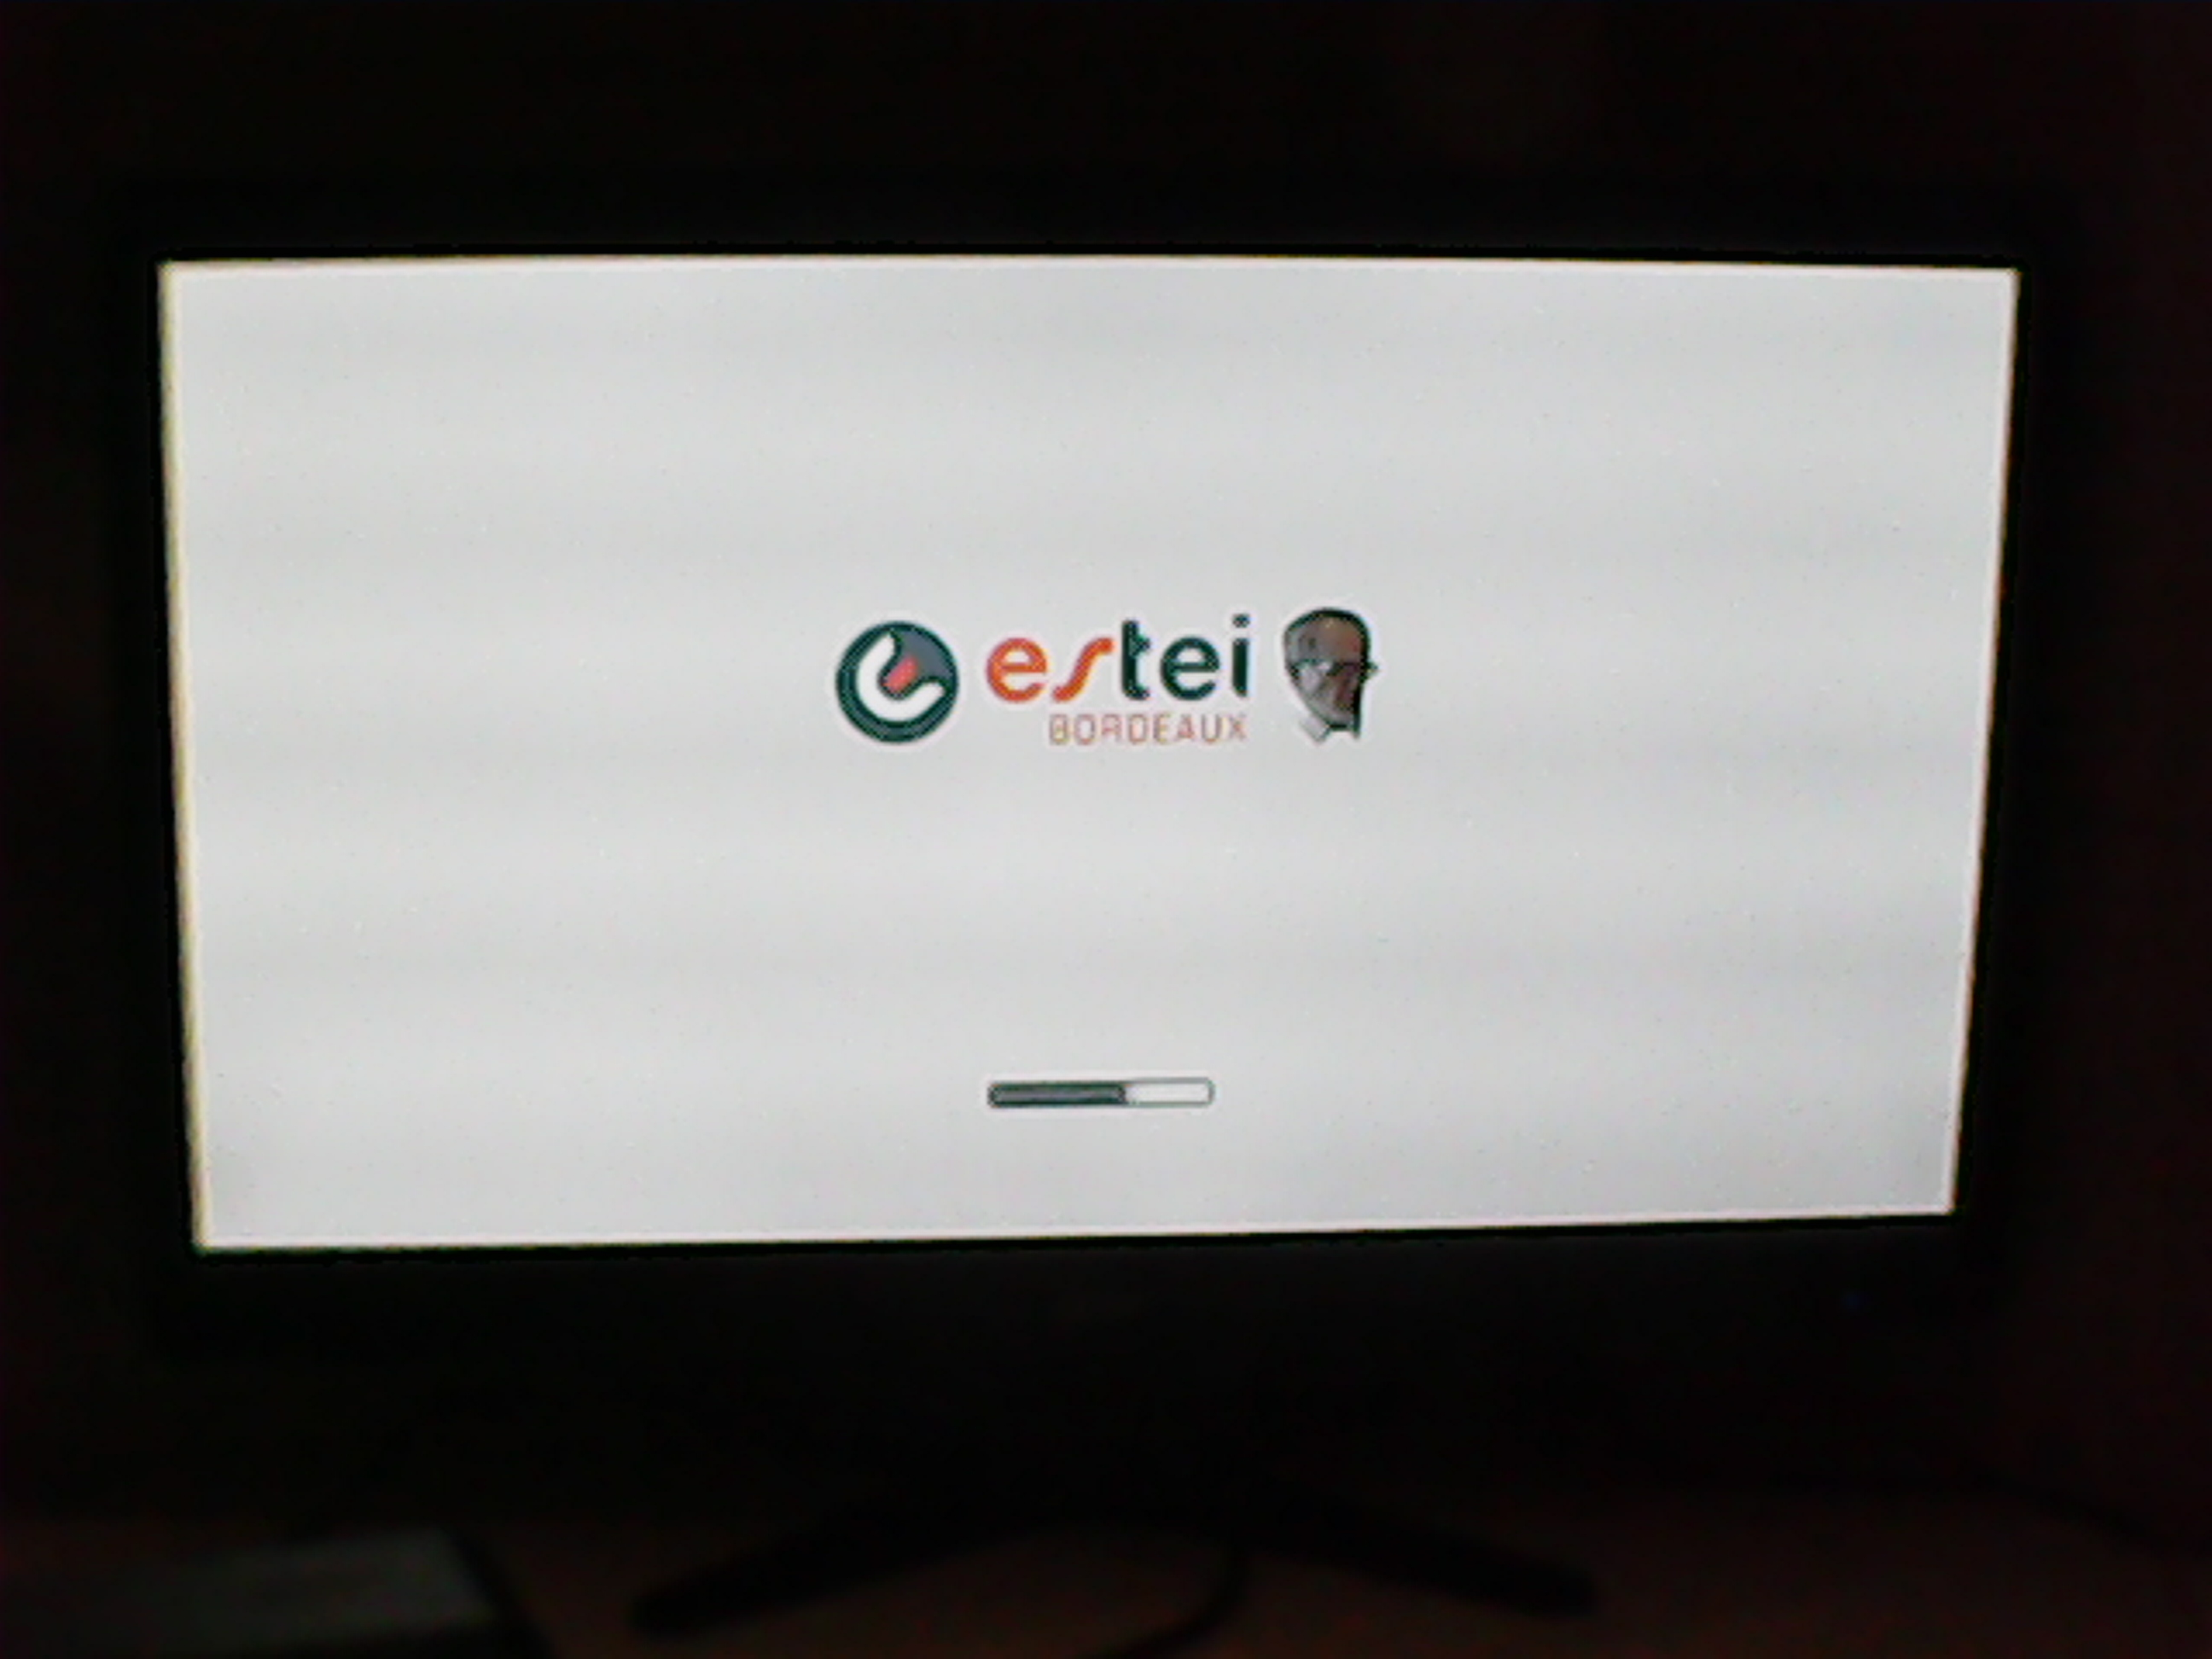
\includegraphics[width=0.49\linewidth]{\figures/photo_splashi_1.jpg}
    \decoRule
    \caption[
    Écrans de démarrage du noyau Linux à droite et du processus d'initialisation à gauche]{
    Écrans de démarrage du noyau Linux à droite et du processus d'initialisation à gauche}
    \label{fig:Écrans de démarrage du noyau Linux à droite et du processus d'initialisation à gauche}
    \end{figure}

\vspace{1cm}

Les messages provenant du kernel s'affichent par dessus l'écran de démarrage et "polluent" l'écran d'accueil. Il est possible de les masquer en passant l'argument \codeinline{text}{quiet} au kernel lorsque le bootloader l'invoque. L'argument \codeinline{text}{console=tty2} permet de rediriger les messages provenant du processus d'initialisation vers la console \codeinline{text}{/dev/tty2} accessible par la combinaison de touches \codeinline{text}{[CTRL]}, \codeinline{text}{[ALT]}, \codeinline{text}{[F2]}.

Sur Raspberry-Pi, les arguments passés au kernel sont partiellement stockés dans le fichier \codeinline{text}{cmdline.txt}. Pour le modifier depuis Yocto, on ajoute la ligne suivante à la recette

\mintinline[fontsize=\footnotesize]{text}{meta-autoscope/recipes-kernel/linux/linux-raspberrypi_%.bbappend}~:
\code{bash}
CMDLINE_append = "quiet console=tty2"
\end{minted}

\begin{figure}[H]
    \centering
    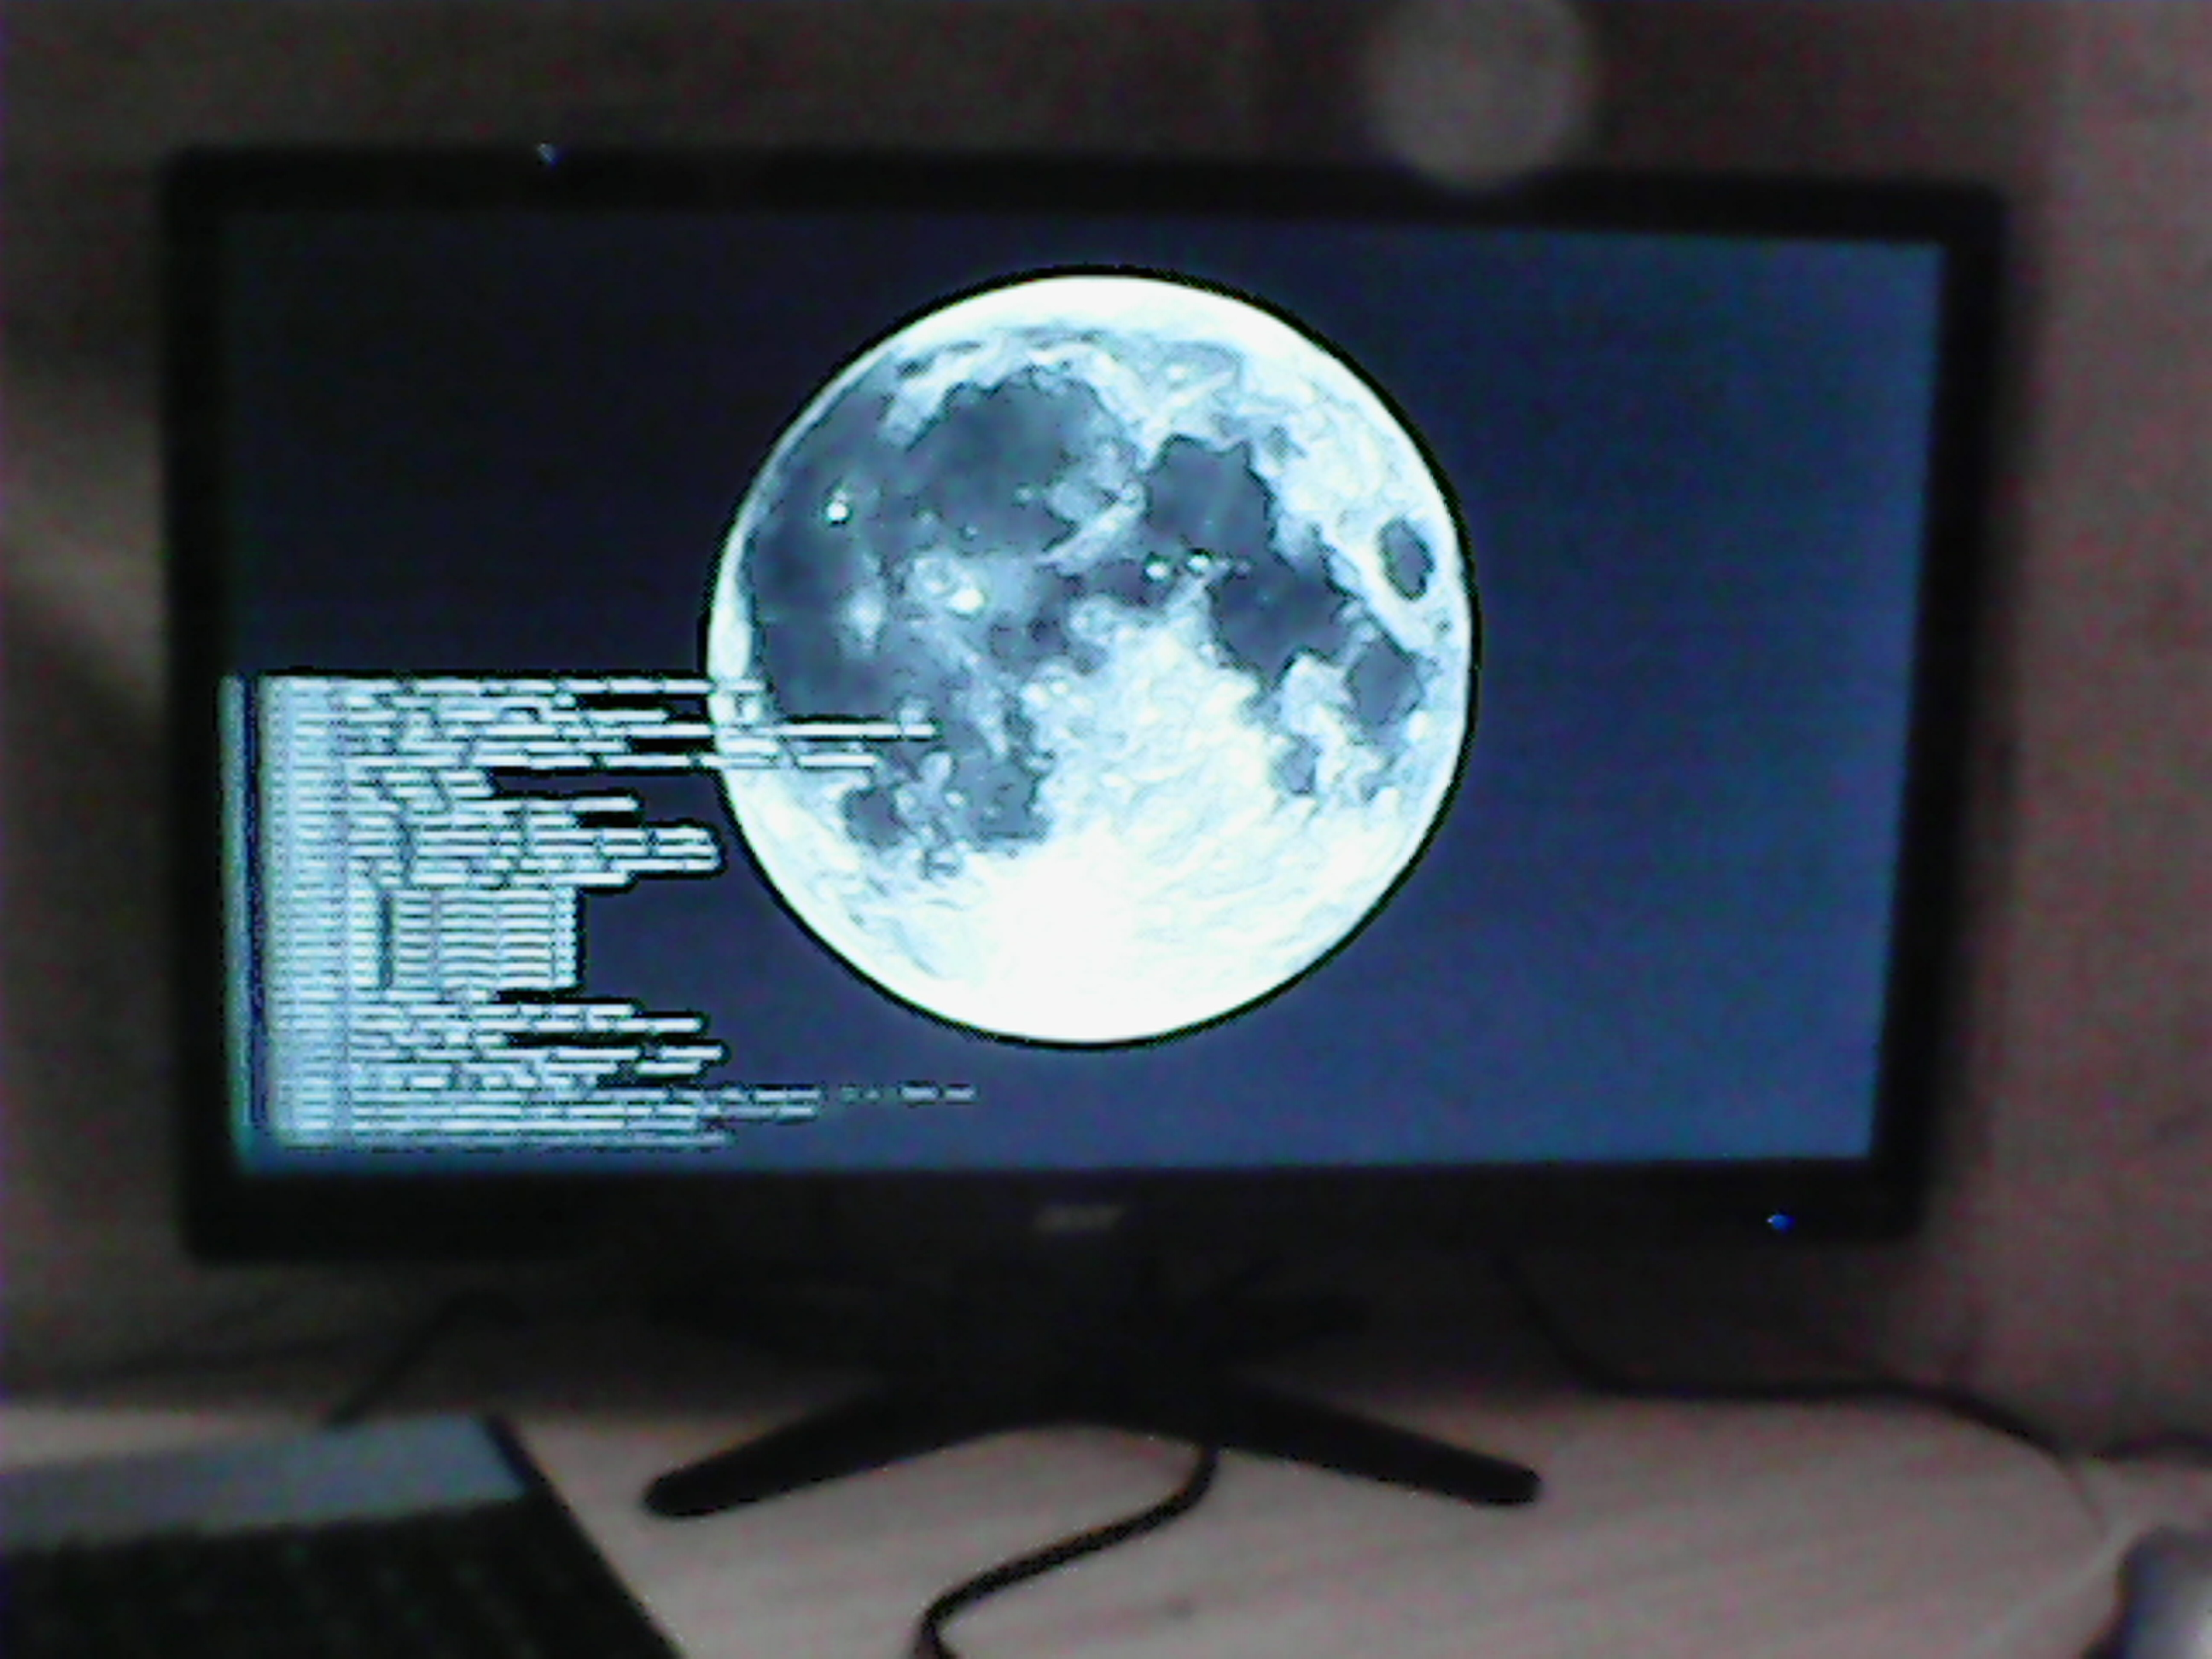
\includegraphics[width=0.49\linewidth]{\figures/photo_splashk_3.jpg}
    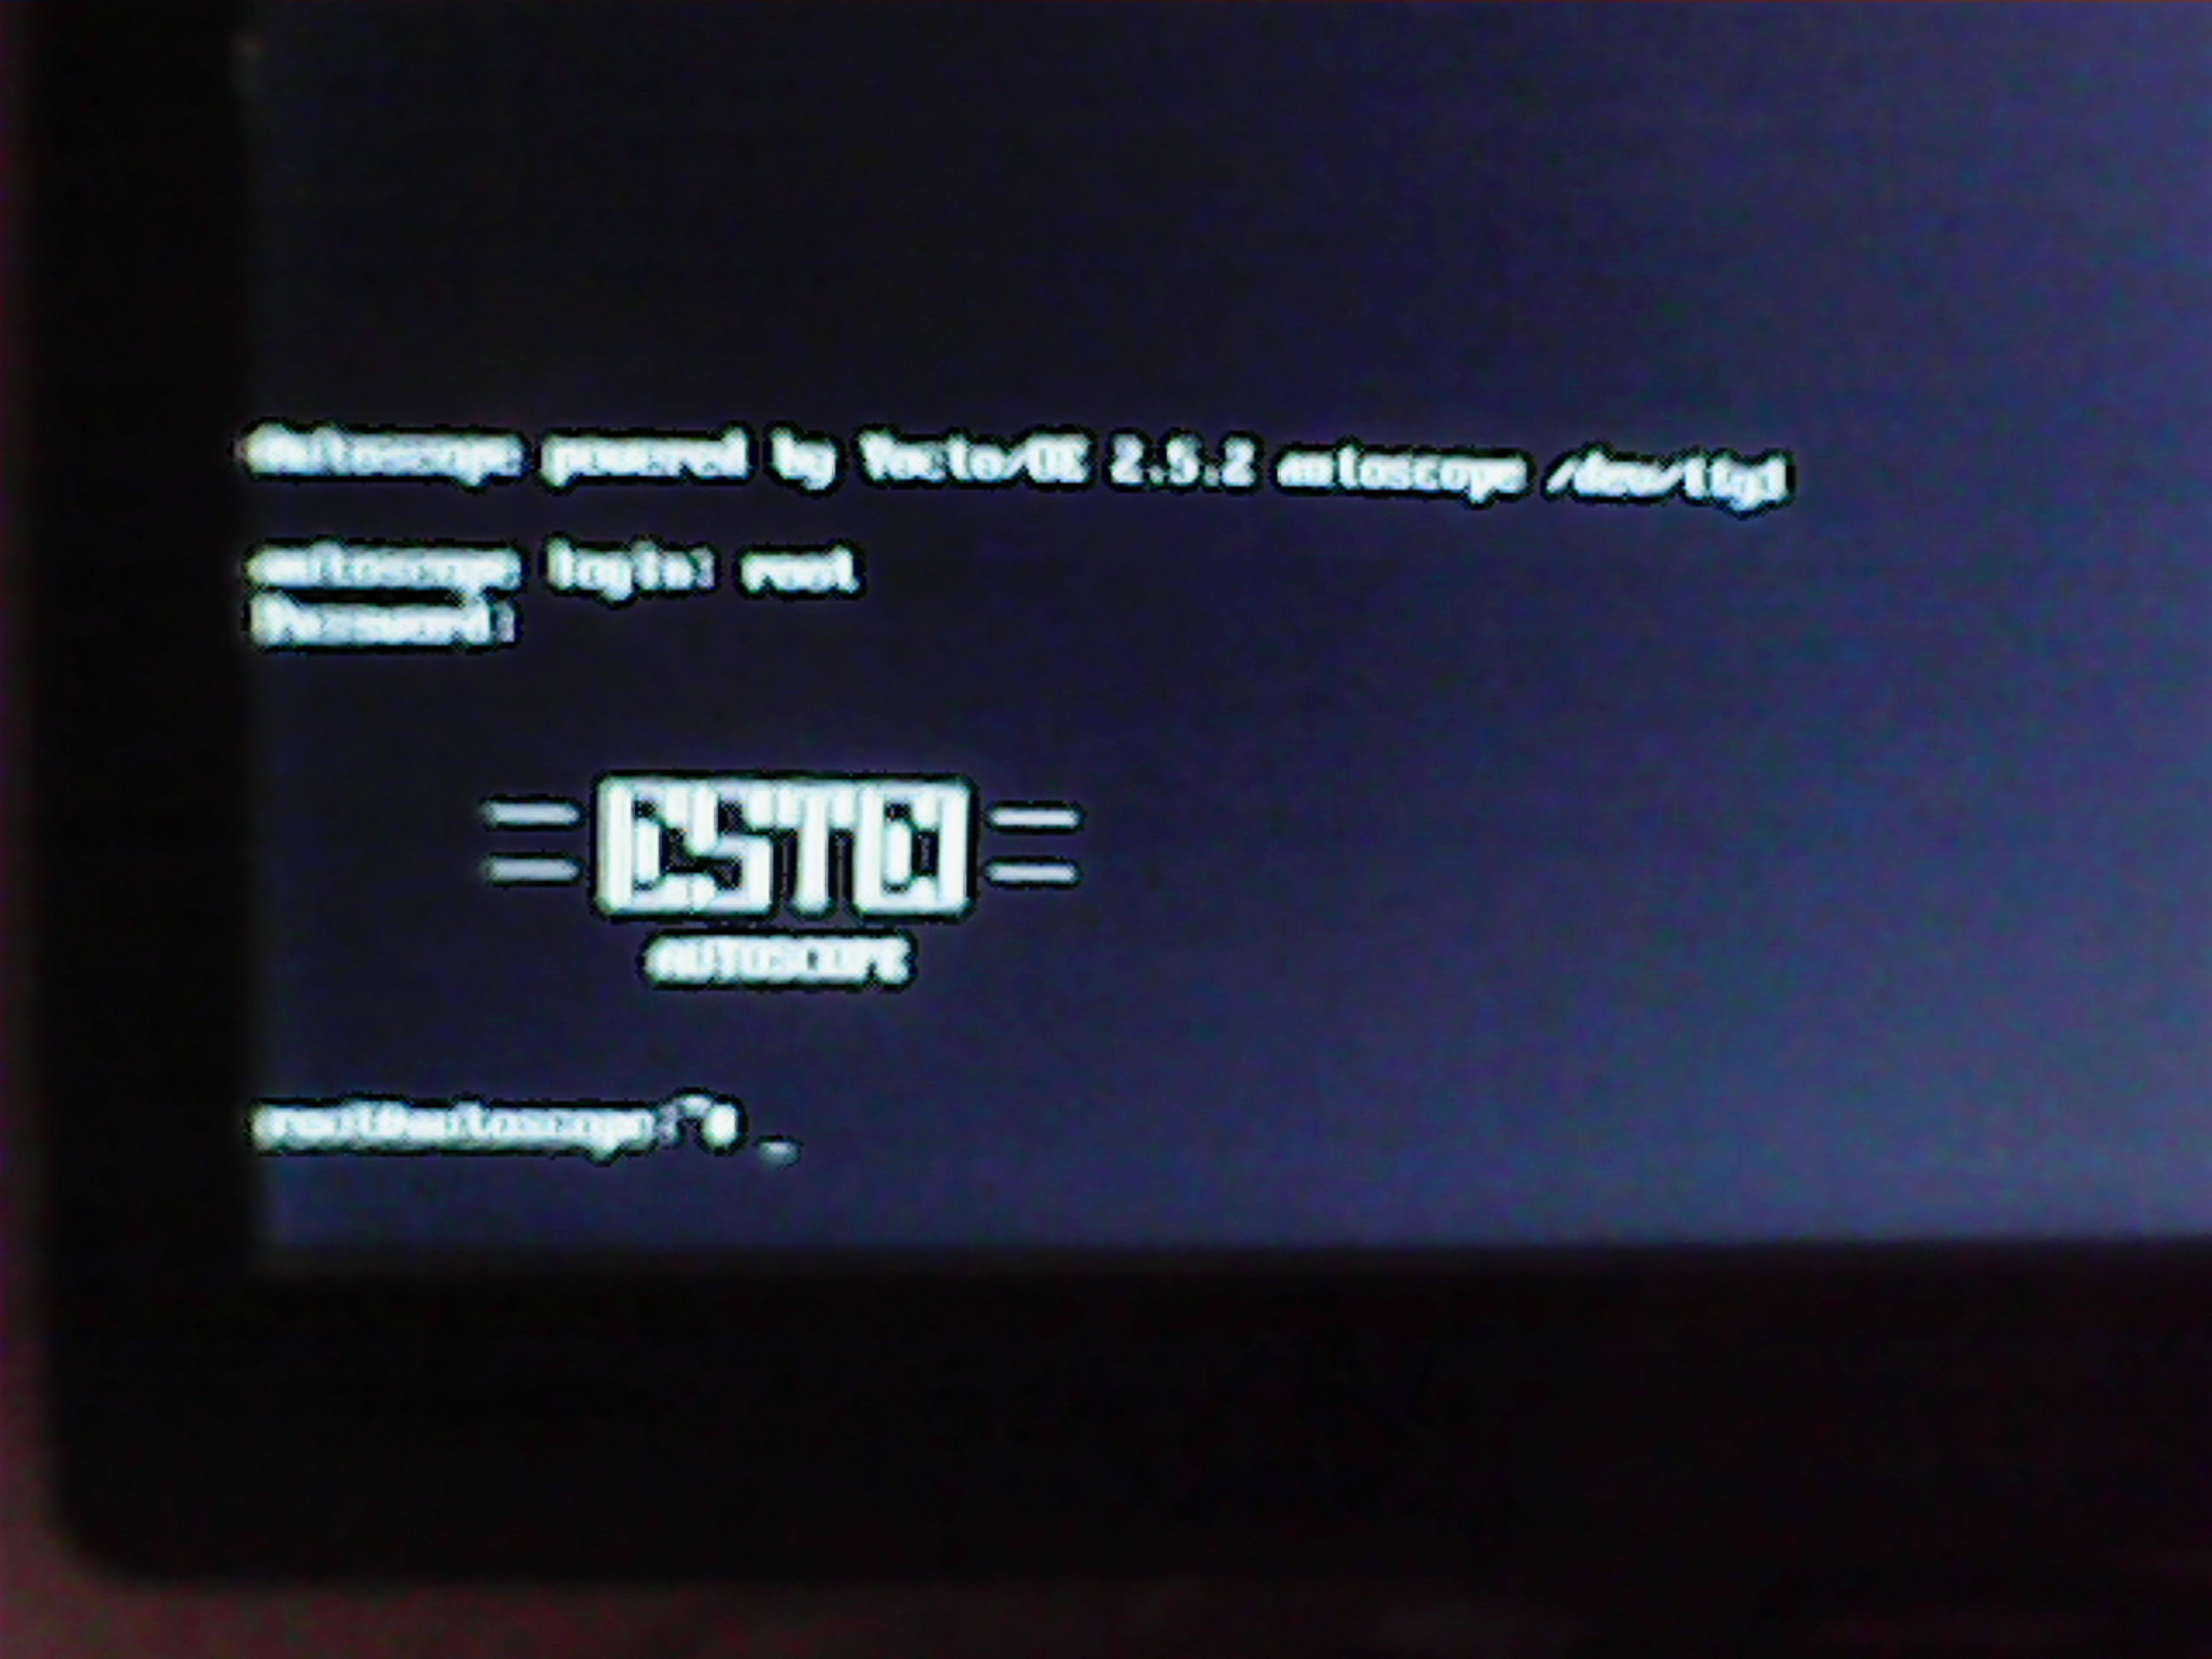
\includegraphics[width=0.49\linewidth]{\figures/photo_log_1.jpg}
    \decoRule
    \caption[
    Écran de démarrage du noyau Linux à droite et écran d'accueil à gauche]{
    Écran de démarrage du noyau Linux à droite et écran d'accueil à gauche}
    \label{fig:Écran de démarrage du noyau Linux à droite et écran d'accueil à gauche}
    \end{figure}

\section{Hotspot Wifi}

Configurer le télescope en Hotspot Wifi est une solution intéressante car ainsi un appareil client peut s'y connecter sans qu'il n'y ait besoin d'une infrastructure existante, un réseau local par exemple.

Pour configurer la Raspberry-Pi en Hotspot, deux choses sont nécessaires~:
\begin{itemize}[label=$\bullet$]
	\item Configurer le kernel pour qu'il supporte le mode \codeinline{text}{tether}.
	\item Le logiciel \codeinline{text}{connman}
	\end{itemize}

\codeinline{text}{meta-autoscope/recipes-kernel/linux/linux-raspberrypi/raspberrypi3/hotspot.cfg}~:
\code{c}
CONFIG_BRIDGE=m
CONFIG_IP_NF_TARGET_MASQUERADE=m
CONFIG_NETFILTER=m
CONFIG_NF_CONNTRACK_IPV4=m
CONFIG_NF_NAT_IPV4=m

CONFIG_IP_NF_IPTABLES=m
CONFIG_IP_MULTIPLE_TABLES=m
CONFIG_NETFILTER_NETLINK_ACCT=m
CONFIG_NETFILTER_XT_MATCH_NFACCT=m
CONFIG_NETFILTER_XT_CONNMARK=m
CONFIG_NETFILTER_XT_TARGET_CONNMARK=m
CONFIG_NETFILTER_XT_MATCH_CONNMARK=m
\end{minted}

\mintinline[fontsize=\footnotesize]{text}{meta-autoscope/recipes-kernel/linux/linux-raspberrypi_%.bbappend}~:
\code{bash}
SRC_URI_append_raspberrypi3 += " \
    file://0001-Autoscope-logo.patch \
    file://logo.cfg \
    file://hotspot.cfg \
    file://logo_autoscope_clut224.ppm \
    "
\end{minted}

\codeinline{text}{meta-autoscope/recipes-autoscope/images/autoscope-console-image.bb}~:
\code{bash}
HOTSPOT = " \
    connman \
    connman-client \
    iptables \
"

IMAGE_INSTALL += " \
    ${CAMERA} \
    ${HOTSPOT} \
"
\end{minted}

\vspace{1cm}

Si l'on effectue les commandes suivantes, la Raspberry-Pi devient visible sur le réseau~:
\code{text}
root@autoscope ~ #
    sysctl -w net.ipv4.ip_forward=1
    connmanctl enable wifi
    connmanctl tether wifi on Autoscope 123456789
\end{minted}

\vspace{1cm}

Pour automatiser le processus au démarrage, il faut utiliser le paquet \codeinline{text}{connman-conf} et remplir quelques fichiers de configuration~:

\codeinline{text}{meta-autoscope/recipes-autoscope/images/autoscope-console-image.bb}~:
\code{bash}
HOTSPOT = " \
    connman \
    connman-client \
    connman-conf \
    iptables \
"
\end{minted}

\codeinline{text}{meta-autoscope/recipes-connectivity/connman-conf/files/main.conf}~:
\code{bash}
[General]
DefaultAutoConnectTechnologies=wifi
TetheringTechnologies=wifi
PersistentTetheringMode=true
\end{minted}

\codeinline{text}{meta-autoscope/recipes-connectivity/connman-conf/files/settings}~:
\code{bash}
[global]
OfflineMode=false

[WiFi]
Enable=true
Tethering=true
Tethering.Identifier=Autoscope
Tethering.Passphrase=123456789

[Wired]
Enable=true
Tethering=false

[P2P]
Enable=false
Tethering=false
\end{minted}

\codeinline{text}{meta-autoscope/recipes-connectivity/connman-conf/connman-conf.bbappend}~:
\code{bash}
FILESEXTRAPATHS_prepend := "${THISDIR}/files:"

SRC_URI += " \
    file://main.conf \
    file://settings \
"

FILES_${PN} += "${sysconfdir}/*"

do_install_append() {
    install -d ${D}${sysconfdir}/connman/
    install -m 0755 ${WORKDIR}/main.conf ${D}${sysconfdir}/connman/main.conf
    install -d ${D}${localstatedir}/lib/connman/
    install -m 0755 ${WORKDIR}/settings ${D}${localstatedir}/lib/connman/settings
}
\end{minted}

Les lignes ajoutées à \codeinline{text}{do_install()} permettent de déplacer les fichiers à leur place dans l'arborescence du système~:
\begin{itemize}[label=$\bullet$]
	\item \codeinline{text}{/etc/connman/main.conf}
	\item \codeinline{text}{/var/lib/connman/settings}
	\end{itemize}

\vspace{1cm}

À noter que sans la ligne \codeinline{text}{FILES_${PN} += "${sysconfdir}/*"}, Bitbake est incapable de connaître cette variable et donc de déplacer le fichier. La question ne se pose pas pour la variable \codeinline{text}{localstatedir} puisque l'on trouve la ligne suivante\\\codeinline{text}{FILES_${PN} = "${localstatedir}/* ${datadir}/*"} dans la recette originale~:\\\codeinline{text}{poky/meta/recipes-connectivity/connman-conf/connman-conf.bb}

\vspace{1cm}

Quant à la commande \codeinline{text}{sysctl -w net.ipv4.ip_forward=1} qui n'est pas à effectuer à chaque démarrage, on peut l'automatiser ainsi~:

\codeinline{text}{meta-autoscope/recipes-autoscope/images/autoscope-console-image.bb}~:
\code{bash}
hotspot() {
    echo 'net.ipv4.ip_forward = 1' >> ${IMAGE_ROOTFS}/etc/sysctl.conf
}

ROOTFS_POSTPROCESS_COMMAND += " hotspot; "
\end{minted}

\vspace{1cm}

Ainsi, dès le démarrage de la Raspberry-Pi, le Hotspot \codeinline{text}{Autoscope} est visible depuis un équipement Wifi. Le mot de passe est \codeinline{text}{123456789}.

\begin{figure}[H]
    \centering
    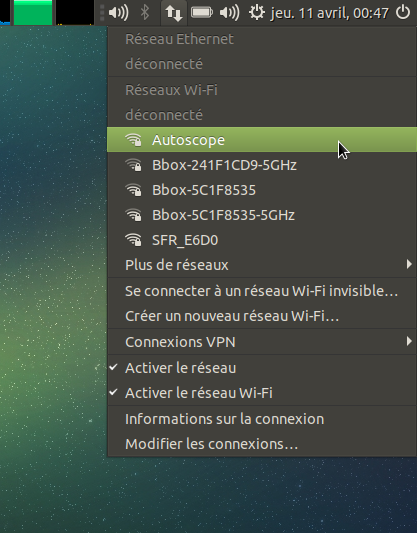
\includegraphics[width=0.4\linewidth]{\figures/photo_hotspot.png}
    \decoRule
    \caption[
    Connexion à la Raspberry-Pi depuis un ordinateur distant]{
    Connexion à la Raspberry-Pi depuis un ordinateur distant}
    \label{fig:Connexion à la Raspberry-Pi depuis un ordinateur distant}
    \end{figure}

\section{Serveur FTP}

Plusieurs serveurs FTP sont disponibles dans Poky, \codeinline{text}{vsftpd} semble être une bonne solution pour sa légèreté, sa fiabilité et ses possibilités de configuration.

\codeinline{text}{meta-autoscope/recipes-autoscope/images/autoscope-console-image.bb}~:
\code{bash}
FTP = " \
    vsftpd \
"

IMAGE_INSTALL += " \
    ${CAMERA} \
    ${HOTSPOT} \
    ${FTP} \
"
\end{minted}

\codeinline{text}{meta-autoscope/recipes-connectivity/vsftpd/vsftpd_\%.bbappend}~:
\code{bash}
FILESEXTRAPATHS_prepend := "${THISDIR}/files:"
\end{minted}

\codeinline{text}{meta-autoscope/recipes-connectivity/vsftpd/files/vsftpd.user_list}~:
\code{bash}
autoscope
\end{minted}

\codeinline{text}{meta-autoscope/recipes-connectivity/vsftpd/files/vsftpd.conf}~:
\code{bash}
listen=YES
anonymous_enable=NO
local_enable=YES
write_enable=YES
local_umask=022
dirmessage_enable=YES
xferlog_enable=YES
connect_from_port_20=YES
xferlog_std_format=YES
ftpd_banner=Welcome to Autoscope FTP service.
ls_recurse_enable=YES
pam_service_name=vsftpd
userlist_deny=NO
userlist_enable=YES
use_localtime=YES
chroot_local_user=YES
allow_writeable_chroot=YES
tcp_wrappers=YES
user_sub_token=$USER
local_root=/home/$USER
\end{minted}

Note~: Des commentaires explicatifs figurent dans le fichier \codeinline{text}{vsftpd.conf} mais ne sont pas affichés ici.

\vspace{1cm}

Le serveur est alors accessible depuis un navigateur web via l'URL \codeinline{text}{ftp://<ip.raspberry.pi>} ou plus simplement la commande \codeinline{text}{ftp autoscope@<ip.raspberry.pi>}. Le mot de passe de l'utilisateur \codeinline{text}{autoscope} est demandé.

\begin{figure}[H]
    \centering
    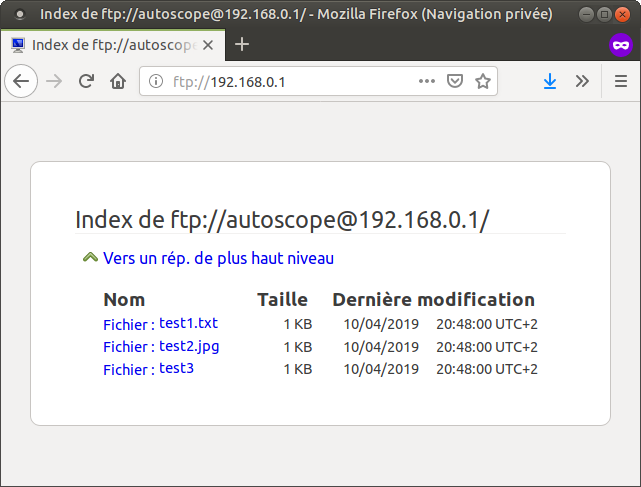
\includegraphics[width=0.7\linewidth]{\figures/photo_ftp.png}
    \decoRule
    \caption[
    Accès au serveur FTP de la Raspberry-Pi depuis un navigateur]{
    Accès au serveur FTP de la Raspberry-Pi depuis un navigateur}
    \label{fig:Accès au serveur FTP de la Raspberry-Pi depuis un navigateur}
    \end{figure}

\vspace{1cm}

\begin{itemize}[label=$\bullet$]
	\item \codeinline{text}{autoscope} est le seul utilisateur autorisé à accéder au serveur FTP.
	\item Le serveur se lance automatiquement lors de la phase d'initialisation du système.
	\item L'option \codeinline{text}{chroot_local_user=YES} du fichier \codeinline{text}{vsftpd.conf} empêche l'utilisateur de remonter dans l'arborescence du système au delà du dossier défini par l'option\\\codeinline{text}{local_root=/home/$USER}, c'est-à-dire \codeinline{text}{/home/autoscope}. Il s'agit là d'une mesure élémentaire de sécurité.
	\end{itemize}

\section{Driver helloworld}

Ce driver minimaliste a pour but de préparer le terrain pour les drivers des moteurs, du GPS et de l'IMU.

\codeinline{text}{hello.c}~:
\code{C}
#include <linux/module.h>

int init_module(void)
{
    printk("Hello World!\n");
    return 0;
}

void cleanup_module(void)
{
    printk("Goodbye Cruel World!\n");
}

MODULE_LICENSE("GPL");
\end{minted}

\codeinline{text}{Makefile}~:
\code{makefile}
obj-m := hello.o

SRC := $(shell pwd)

all:
    $(MAKE) -C $(KERNEL_SRC) M=$(SRC)

modules_install:
    $(MAKE) -C $(KERNEL_SRC) M=$(SRC) modules_install

clean:
    rm -f *.o *~ core .depend .*.cmd *.ko *.mod.c
    rm -f Module.markers Module.symvers modules.order
    rm -rf .tmp_versions Modules.symvers
\end{minted}

Un fichier \codeinline{text}{COPYING} contient une licence GPL.

\vspace{1cm}

Tous ces fichiers figurent sur une branche dédiée \codeinline{text}{hello_mod} du dépôt~:\\\codeinline{text}{github.com/thibaudledo/Autoscope}.

\vspace{1cm}

\codeinline{text}{meta-autoscope/recipes-test/hello-mod/hello-mod_git.bb}~:
\code{bash}
SUMMARY = "Example of how to build an external Linux kernel module"
LICENSE = "GPLv2"
LIC_FILES_CHKSUM = "file://${COREBASE}/meta/COPYING.GPLv2;md5=751419260aa954499f7abaabaa882bbe"

inherit module

SRC_URI = "git://github.com/thibaudledo/Autoscope;protocol=git;branch=hello_mod"

SRCREV = "${AUTOREV}"
S = "${WORKDIR}/git"

RPROVIDES_${PN} += "kernel-module-hello"
\end{minted}

\codeinline{text}{meta-autiscope/recipes-autoscope/images/autoscope-console-image.bb}~:
\code{bash}
HELLOWORLD = " \
    hello-mod \
" 

IMAGE_INSTALL += " \
    ${CAMERA} \
    ${HOTSPOT} \
    ${FTP} \
    ${HELLOWORLD} \
"
\end{minted}

\vspace{1cm}

Ainsi avec les commandes suivantes on observe les messages d'init et de cleanup s'afficher~:
\code{text}
root@autoscope ~ #
    modprobe hello
        [  xx.xxxxxx] hello: loading out-of-tree module taints kernel.
        [  xx.xxxxxx] Hello World!
    rmmod hello
        [  xx.xxxxxx] Goodbye Cruel World!
\end{minted}

\section{Programme helloworld}

Ce programme a pour but de préparer le terrain pour le programme principal du télescope ainsi que pour d'éventuels programmes de test.

\codeinline{text}{meta-autoscope/recipes-test/helloworld/files/helloworld.c}~:
\code{c}
#include <stdio.h>
#include <unistd.h>

int main(void) {
    while(1) {
        printf("helloworld : TEST MESSAGE\n");
        usleep(2000000);
        }
    return(0);
    }
\end{minted}

\vspace{1cm}

En l'absence de \codeinline{text}{Makefile}, c'est à la recette de comporter les instructions de compilation du programme.

\codeinline{text}{meta-autoscope/recipes-test/helloworld/helloworld.bb}~:
\code{bash}
SUMMARY = "Helloworld program test"
SECTION = "base"
LICENSE = "GPLv2"
LIC_FILES_CHKSUM = "file://${COREBASE}/meta/COPYING.GPLv2;md5=751419260aa954499f7abaabaa882bbe"

SRC_URI = " \
    file://helloworld.c \
    "

do_compile () {
    ${CC} ${CFLAGS} ${LDFLAGS} ${WORKDIR}/helloworld.c -o ${WORKDIR}/helloworld
}

do_install () {
    install -d ${D}${bindir}
    install -m 0755 ${WORKDIR}/helloworld ${D}${bindir}/
}
\end{minted}

\codeinline{text}{meta-autiscope/recipes-autoscope/images/autoscope-console-image.bb}~:
\code{bash}
HELLOWORLD = " \
    hello-mod \
    helloworld \
" 

IMAGE_INSTALL += " \
    ${CAMERA} \
    ${HOTSPOT} \
    ${FTP} \
    ${HELLOWORLD} \
"
\end{minted}

\vspace{1cm}

À l'issue de la compilation on observe la présence du programme dans le dossier \codeinline{text}{/usr/bin} du \codeinline{text}{rootfs}~:

\code{text}
~/yocto/build/tmp/work/raspberrypi3-poky-linux-gnueabi/autoscope-console-image/1.0-r0/ rootfs $
    find . | grep helloworld
        ./usr/bin/helloworld
\end{minted}

Et à l'usage~:

\code{text}
root@autoscope ~ #
    helloworld
        helloworld : TEST MESSAGE
        helloworld : TEST MESSAGE
        helloworld : TEST MESSAGE
    ^C
\end{minted}

\section{Daemonisation du programme helloworld}

Pour faire d'un programme un daemon, c'est-à-dire un programme se lançant au démarrage de la machine et fonctionnant en tache de fond (comme le serveur FTP par exemple), il faut avoir recours au système d'initialisation de l'OS, ici il s'agit de SysVinit.

\vspace{1cm}

On écrit d'abord un script d'initialisation qui sera installé dans le dossier \codeinline{text}{/etc/init.d/} doté un bandeau d'entête où figurent notamment les runlevels dans lesquels le daemon doit être invoqué et ceux dans lesquels il doit être tué. Généralement un daemon peut être invoqué dans les runlevels $2$, $3$, $4$, $5$ et peut être tué dans les runlevels $0$, $1$, $6$. Généralement le runlevel $5$ est celui de fonctionnement normal de la machine, $0$ celui de l'arrêt et $6$ celui du redémarrage.

\codeinline{text}{meta-autoscope/recipes-test/helloworld/files/helloworld.sh}~:
\code{bash}
#!/bin/sh
### BEGIN INIT INFO
# Provides:             helloworld
# Required-Start:
# Required-Stop:
# Default-Start:        5
# Default-Stop:         0 1 6
# Short-Description:    Helloworld test
### END INIT INFO

NAME="helloworld"
DESC="Test program"
DAEMON="/usr/bin/${NAME}"

case "$1" in
    start)
        echo -n "Starting ${DESC}: ${NAME}... "
#       start-stop-daemon -S -b -C -q -x ${DAEMON} > /dev/tty3 #-C don't work with busybox
        ${DAEMON} > /dev/tty3 &
        echo "done"
        ;;
    stop)
        echo -n "Stopping ${DESC}: ${NAME}... "
        start-stop-daemon -K -q -x ${DAEMON}
        echo "done"
        ;;
    restart)
        $0 stop
        $0 start
        ;;
    status)
        start-stop-daemon -T -q -x ${DAEMON}
        case "$?" in
            0)
                echo "Program ${NAME} is running (`pidof ${NAME}`)."
                ;;
            1)
                echo "Programm ${NAME} is not running and the pid file exists."
                ;;
            3)
                echo "Programm ${NAME} is not running."
                ;;
            4)
                echo "Unable to determine ${NAME} status."
                ;;
            esac
        ;;
    *)
        echo "Usage: $0 {start|stop|restart|status}"
        exit 1
        ;;
    esac
exit 0
\end{minted}

Les messages produits par le daemon sont redirigés vers la console \codeinline{text}{/dev/tty3} accessible par la combinaison de touches \codeinline{text}{[CTRL]}, \codeinline{text}{[ALT]}, \codeinline{text}{[F3]}.

\vspace{1cm}

La recette yocto est légèrement différente.

\codeinline{text}{meta-autoscope/recipes-test/helloworld/helloworld-daemon.bb}~:
\code{bash}
SUMMARY = "Helloworld daemon test"
SECTION = "base"
LICENSE = "GPLv2"
LIC_FILES_CHKSUM = "file://${COREBASE}/meta/COPYING.GPLv2;md5=751419260aa954499f7abaabaa882bbe"

SRC_URI = " \
    file://helloworld.sh \
    file://helloworld.c \
    "
inherit update-rc.d

do_compile () {
    ${CC} ${CFLAGS} ${LDFLAGS} ${WORKDIR}/helloworld.c -o ${WORKDIR}/helloworld
}

do_install () {
    install -d ${D}${sysconfdir}/init.d
    cat ${WORKDIR}/helloworld.sh | \
      sed -e 's,/etc,${sysconfdir},g' \
          -e 's,/usr/sbin,${sbindir},g' \
          -e 's,/var,${localstatedir},g' \
          -e 's,/usr/bin,${bindir},g' \
          -e 's,/usr,${prefix},g' > ${D}${sysconfdir}/init.d/helloworld
    chmod a+x ${D}${sysconfdir}/init.d/helloworld

    install -d ${D}${bindir}
    install -m 0755 ${WORKDIR}/helloworld ${D}${bindir}/
}

INITSCRIPT_NAME = "helloworld"
INITSCRIPT_PARAMS = "start 99 5 . stop 00 0 1 6 ."
\end{minted}

\codeinline{text}{meta-autiscope/recipes-autoscope/images/autoscope-console-image.bb}~:
\code{bash}
HELLOWORLD = " \
    hello-mod \
    helloworld-daemon \
" 

IMAGE_INSTALL += " \
    ${CAMERA} \
    ${HOTSPOT} \
    ${FTP} \
    ${HELLOWORLD} \
"
\end{minted}

\vspace{1cm}

On observe ensuite dans le \codeinline{text}{rootfs} la présence du script d'initialisation ainsi que la présence d'un lien symbolique vers celui-ci dans les dossiers des runlevels 0, 1, 5, 6 avec des préfixes~:
\begin{itemize}[label=$\bullet$]
	\item \codeinline{text}{S} ou \codeinline{text}{K} indiquant si le daemon est invoqué (Start) ou tué (Kill).
	\item \codeinline{text}{00} à \codeinline{text}{99} indiquant le numéro de priorité de l'appel, \codeinline{text}{00} étant le plus prioritaire.
	\end{itemize}

\code{text}
~/yocto/build/tmp/work/raspberrypi3-poky-linux-gnueabi/autoscope-console-image/1.0-r0/ rootfs $
    find . | grep helloworld
        ./usr/bin/helloworld
        ./etc/init.d/helloworld
        ./etc/rc0.d/K00helloworld
        ./etc/rc1.d/K00helloworld
        ./etc/rc5.d/S99helloworld
        ./etc/rc6.d/K00helloworld
\end{minted}

\vspace{1cm}

Et à l'usage~:

\code{text}
root@autoscope ~ #
    /etc/init.d/helloworld status
        Program helloworld is running (347).

    # [CTRL] [ALT] [F3]
        helloworld : TEST MESSAGE
        helloworld : TEST MESSAGE
        helloworld : TEST MESSAGE

    # [CTRL] [ALT] [F1]
    /etc/init.d/helloworld stop
        Stopping Test program: helloworld... done
    /etc/init.d/helloworld status
        Program helloworld is not running.
\end{minted}

\section{Support de la liaison UART}

Pour activer le support de la liaison UART, il faut ajouter la ligne suivante au fichier \codeinline{text}{config.txt}
\code{bash}
enable_uart=1
\end{minted}

C'est-à-dire la ligne suivante à la recette

\mintinline[fontsize=\footnotesize]{text}{meta-autoscope/recipes-bsp/bootfiles/rpi-config_%.bbappend}~:
\code{bash}
ENABLE_UART = "1"
\end{minted}

Remarque~: Ce genre de variables de configurations propre aux Raspberry-Pi est généralement utilisé via les fichiers \codeinline{text}{local.conf} ou \codeinline{text}{distro.conf}. La raison en est que certaines, comme \codeinline{text}{ENABLE_UART} justement, ont un effet dans plusieurs recettes. Celle-ci, par le biais de la recette \mintinline[fontsize=\footnotesize]{text}{linux-raspberrypi_%.bb} ajoute également \codeinline{text}{console=serial0,115200} au fichier \codeinline{text}{cmdline.txt}. Ce fichier contient les arguments qu'U-Boot passe à Linux lorsqu'il l'appelle. Dans notre cas cette ligne n'est pas souhaitable, on peut donc placer la variable dans une surcharge de la recette \mintinline[fontsize=\footnotesize]{text}{rpi-config_%.bb}

\vspace{1cm}

On observe que désormais le fichier \codeinline{text}{/dev/ttyS0} existe, avant cela seul \codeinline{text}{/dev/ttyAMA0} existait, autre ligne UART utilisée par le module Bluetooth de la Raspberry-pi.

Si l'on boucle la ligne \codeinline{text}{Tx} sur \codeinline{text}{Rx} et que l'on observe à l'analyseur logique, voici la trame observée pour une écriture quelconque sur la ligne.

\code{text}
root@autoscope ~ #
    echo "5A" | microcom /dev/ttyS0 -s 9600
        5A
\end{minted}

\begin{figure}[H]
    \centering
    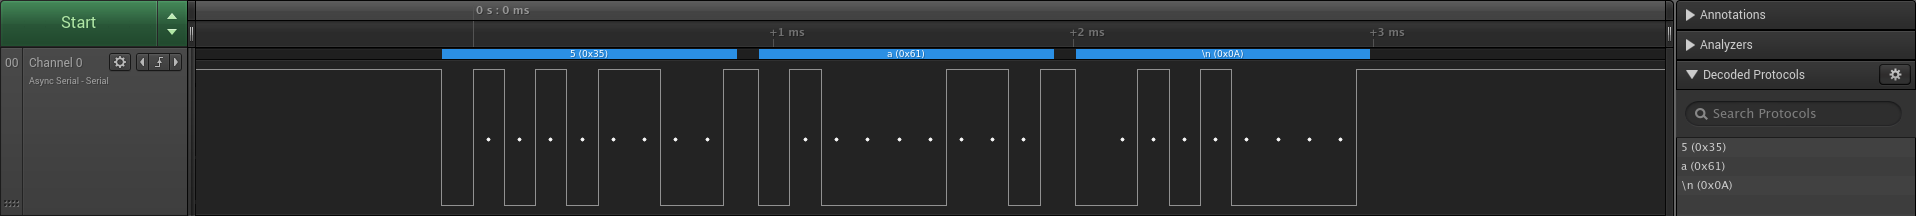
\includegraphics[width=1\linewidth]{\figures/osc_uart.png}
    \decoRule
    \caption[
    Trame UART relevée à l'analyseur logique]{
    Trame UART relevée à l'analyseur logique}
    \label{fig:Trame UART relevée à l'analyseur logique}
    \end{figure}

\vspace{1cm}

On retrouve les trois caractères ASCII envoyés par la commande \codeinline{text}{echo}. Ceux-ci réapparaissant également à l'écran, démontrant le fonctionnement de la liaison en lecture et en écriture.

\section{Support du bus I2C et communication avec l'IMU}

Pour activer le support du bus I2C, il faut ajouter les lignes suivantes au fichier \codeinline{text}{config.txt}
\code{bash}
dtparam=i2c1=on
dtparam=i2c_arm=on
\end{minted}

C'est-à-dire la ligne suivante à la recette

\mintinline[fontsize=\footnotesize]{text}{meta-autoscope/recipes-bsp/bootfiles/rpi-config_%.bbappend}~:
\code{bash}
ENABLE_I2C = "1"
\end{minted}

\vspace{1cm}

On ajoute également la suite de test \codeinline{text}{i2c-tools}~:

\codeinline{text}{meta-autoscope/recipes-autoscope/images/autoscope-console-image.bb}~:
\code{bash}
IMAGE_INSTALL += " \
    ${CAMERA} \
    ${HOTSPOT} \
    ${FTP} \
    ${HELLOWORLD} \
    i2c-tools \
"
\end{minted}

\vspace{1cm}

Ensuite, pour pouvoir utiliser \codeinline{text}{i2c-tools}, il faut activer un driver~:

\code{text}
root@autoscope ~ #
    modprobe i2c_dev
        [  xx.xxxxxx] i2c /dev entries driver
\end{minted}

Remarque~: Il est possible de le charger dès le démarrage en utilisant la variable\\\codeinline{text}{KERNEL_MODULE_AUTOLOAD}. Celle-ci est utilisable dans la recette kernel ou dans la recette dudit module.

\mintinline[fontsize=\footnotesize]{text}{meta-autoscope/recipes-kernel/linux/linux-raspberrypi_%.bbappend}~:
\code{bash}
KERNEL_MODULE_AUTOLOAD_append = "i2c_dev"
\end{minted}

\vspace{1cm}

On connecte la centrale inertielle au bus I2C et l'on peut observer les périphériques présents sur le bus~:

\code{text}
root@autoscope ~ #
    i2cdetect -y 1
             0  1  2  3  4  5  6  7  8  9  a  b  c  d  e  f
        00:          __ __ __ __ __ __ __ __ __ __ __ __ __
        10: __ __ __ __ __ __ __ __ __ __ __ __ __ __ __ __
        20: __ __ __ __ __ __ __ __ __ __ __ __ __ __ __ __
        30: __ __ __ __ __ __ __ __ __ __ __ __ __ __ __ __
        40: __ __ __ __ __ __ __ __ __ __ __ __ __ __ __ __
        50: __ __ __ __ __ __ __ __ __ __ __ __ __ __ __ __
        60: __ __ __ __ __ __ __ __ 68 __ __ __ __ __ __ __
        70: __ __ __ __ __ __ __ __
\end{minted}

Une seule adresse est attribuée, il s'agit de la centrale inertielle. Il est dit dans sa documentation que le registre \codeinline{text}{WHO_AM_I} à l'adresse \codeinline{text}{0x75} contient invariablement la valeur \codeinline{text}{0x71}. On peut alors essayer de lire ce registre.

\code{text}
root@autoscope ~ #
    i2cget -y 1 0x68 0x75
        0x71
\end{minted}

\begin{figure}[H]
    \centering
    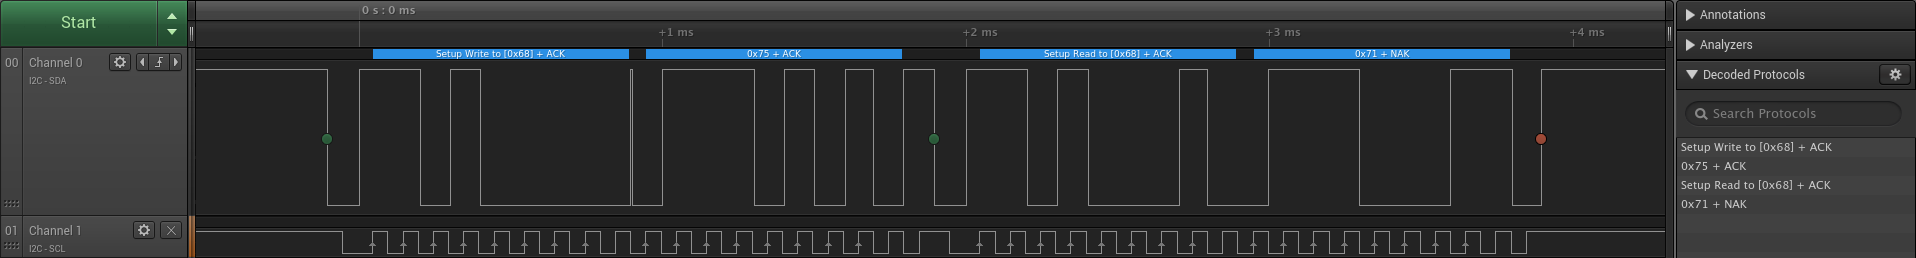
\includegraphics[width=1\linewidth]{\figures/osc_i2c2.png}
    \decoRule
    \caption[
    Trame I2C relevée à l'analyseur logique]{
    Trame I2C relevée à l'analyseur logique}
    \label{fig:Trame I2C relevée à l'analyseur logique}
    \end{figure}

\vspace{1cm}

La communication entre la centrale inertielle et la Raspberry-Pi fonctionne.


